\documentclass[11pt]{article}
\usepackage[a4paper,margin=1in]{geometry}
\usepackage{graphicx}
\usepackage{times}
\usepackage{hyperref}
\usepackage{titlesec}
\usepackage{setspace}
\usepackage{authblk}
\usepackage{amsmath,amssymb}
\graphicspath{{../figures/}{./figures/}}


% Line spacing
\onehalfspacing

% Section style
\titleformat{\section}{\bfseries\large}{\thesection.}{0.5em}{}
\titleformat{\subsection}{\bfseries}{\thesubsection}{0.5em}{}

% Hyperlink color setup
\hypersetup{
    colorlinks=true,
    linkcolor=blue,
    urlcolor=blue,
    citecolor=blue
}

% Title and author info
\title{\textbf{ALL2Vec: Toward a Unified Vector Space Philosophy for Artificial General Intelligence}}
\author{T. Agetaro}
\affil{\textit{Independent Researcher, Japan} \\ \texttt{(contact available via GitHub Issues)}}
\date{October 2025}

\begin{document}
\maketitle

\begin{abstract}
This paper introduces \textbf{"ALL2Vec"}, a conceptual framework proposing that all modalities processed by intelligent systems---language, vision, sound, and other sensory or symbolic data---are fundamentally representable within a \textit{single unified vector space}. The hypothesis arises from the observation that systems based on perceptron-like architectures inevitably interpret input as vectors, implying that any form of cognition, including that of the human brain, operates within a shared vectorized meaning space.

From this perspective, the paper argues that Artificial General Intelligence (AGI) should not treat multimodal processing as the integration of heterogeneous representations, but rather as different projections within one continuous semantic manifold. The \textbf{ALL2Vec} philosophy therefore suggests that the essential step toward AGI is not merely scaling models, but achieving structural unification of meaning through a universal vector space. This framework positions the unified vector space as a fundamental architectural component for future AGI development, aligning with the hypothesis that human consciousness itself arises from such representational coherence.
\end{abstract}

\section{Introduction}
Modern AI architectures, particularly deep learning systems, rely on the transformation of input signals into vector representations. Regardless of the modality—text, image, sound, or motion—each form of data must be represented in a vectorized space to be processed within a neural computational structure. This universality implies a deeper philosophical foundation: the world, as perceived and modeled by such systems, is inevitably mapped into a unified representational continuum.

\section{Background and Motivation}
The notion that ``everything is a vector'' is not new in computational cognition. Word2Vec, Seq2Vec, Doc2Vec, and other embeddings have established that semantic meaning can emerge from distributed representation. However, these models typically operate within modality-specific spaces, requiring additional mechanisms for multimodal integration. 

The \textbf{ALL2Vec} hypothesis generalizes this concept: rather than separate embedding spaces, all perceptual and cognitive data should coexist in a single continuous manifold. This structure reflects not only an engineering convenience but a potential ontological truth about intelligence itself.

\section{Conceptual Framework of ALL2Vec}
ALL2Vec can be expressed conceptually as:
\[
f : \text{All Modalities} \rightarrow \mathbb{R}^n
\]
where $f$ is a mapping from any input modality—language, vision, sound, symbolic structures—into a unified latent vector space $\mathbb{R}^n$.

Within this space, the semantic relationships across different modalities are not arbitrarily aligned but inherently co-expressive. A visual object and its linguistic descriptor, for instance, are neighboring points not through translation but through shared meaning geometry.

\begin{figure}[h!]
    \centering
    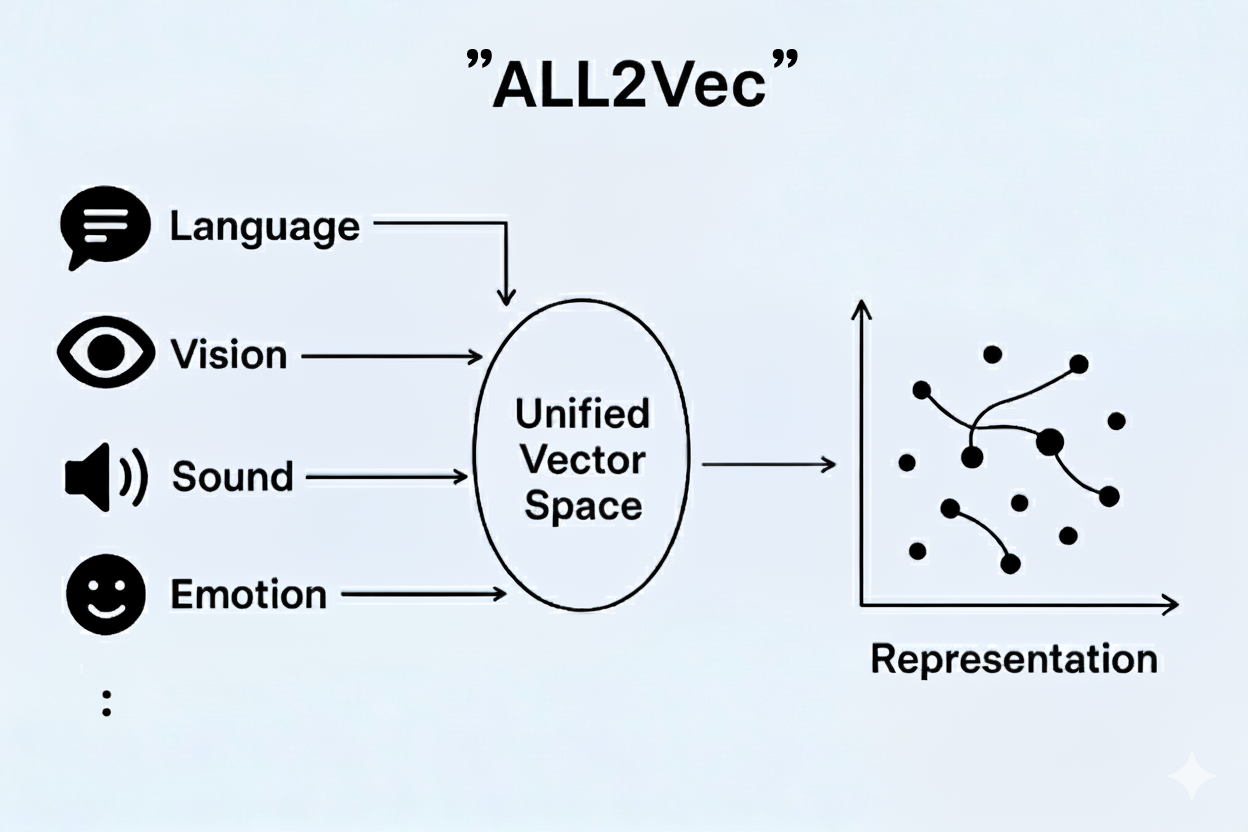
\includegraphics[width=0.85\linewidth]{ALL2Vec_diagram.png}
    \caption{Conceptual illustration of the ``ALL2Vec'' unified vector space. All modalities—language, vision, and sound—map into a single meaning space where cognition emerges as coherent structure.}
\end{figure}

\section{Philosophical Implications}
From a cognitive and philosophical standpoint, ALL2Vec suggests that the coherence of consciousness arises from the unification of representational modalities. If the human brain operates on distributed but convergent neural codes, then its “meaning” might similarly exist as projections on one continuous representational manifold.

Thus, building AGI requires not only computational scalability but the design of an integrated semantic substrate—an architecture where the entire perceptual world is encoded as continuous meaning vectors.

\section{Toward Implementation}
In practical AGI research, this framework motivates several directions:
\begin{itemize}
    \item Unified embeddings where all modalities share common latent bases.
    \item Cross-modal self-supervision enforcing alignment without explicit translation.
    \item Neuromorphic architectures designed to preserve semantic coherence across sensory domains.
\end{itemize}

Such systems could evolve toward a genuinely coherent cognitive substrate rather than a set of disjoint perception modules.

\section{Conclusion}
Based on the hypothesis that the human brain processes all modalities within a unified vector space, this paper proposes the \textbf{ALL2Vec} framework as a foundational architectural principle for AGI. It positions the unified vector space not merely as a computational convenience but as a structural necessity for integrated cognition and consciousness.

\section*{Acknowledgments}
The author thanks the open-source and AI research communities whose work in representation learning laid the foundation for this conceptual study.

\vspace{1em}
\noindent\textbf{Keywords:} Artificial General Intelligence, Unified Representation, Vector Space, Embedding Philosophy, Cognitive Modeling

\end{document}
